%!TEX root = ../thesis.tex

\section{テストフェーズ}

  テストフェーズのシステムを\figref{Fig:RobotGuidance_following_system}に示す.このフェーズでは,学習フェーズで学習したモデルを用いる.つまり,2DLiDARの反射強度を入力としたルールベース制御器の出力ではなく,画像を入力とした深層学習器の出力がロボットの行動を決定する.

  \vspace{0.5cm}

  \begin{figure}[h]
    \centering
    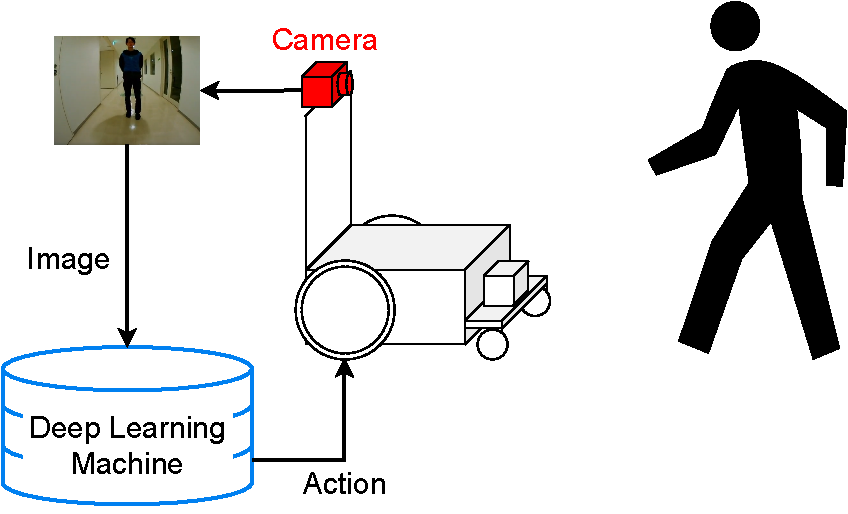
\includegraphics[width=9cm] {images/pdf/RobotGuidance_test_system}
    \captionsetup{justification=raggedright} % キャプションを左寄せに
    \caption{Proposed method in the test phase}
    \label{Fig:RobotGuidance_following_system}
  \end{figure}

  \vspace{0.5cm}

  \begin{figure}[h]
    \centering
    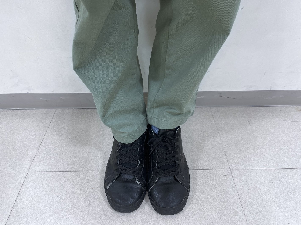
\includegraphics[width=4.5cm] {images/pdf/RobotGuidance_test_phase_leg}
    \captionsetup{justification=raggedright} % キャプションを左寄せに
    \caption{Without retroreflective tape}
    \label{Fig:RobotGuidance_following_phase_leg}
  \end{figure}

\newpage
